\documentclass[20pt]{beamer}
\usepackage{fontspec}
\usepackage{amsfonts}
\usepackage{tangocolors}
\usepackage{setspace}

\usepackage{tikz}
\usetikzlibrary{positioning}
\usetikzlibrary{backgrounds,scopes}
\usetikzlibrary{shapes}

\newcommand\sk{\par\bigskip\bigskip\par}

\newcommand\tl[2]{\texttt{#1}\\\texttt{#2}}

\newcommand\cur{\makebox[0pt]{\textcolor{ta3skyblue!90!black}{\textbar}}}
\newcommand\curc{\cur \textcolor{ta3chameleon}}
\newcommand\nframe[1]{}

\begin{document}
\fontspec{Fertigo Pro}

\begin{center}
\title{Time Warping a synchronizace videí}
\author{Petr Viktorin}
\date{\today}

\frame{
    \texttt{\alt<2->{\textcolor{ta3aluminium}}{}{py}vo}

    \pause
    \bigskip\bigskip\bigskip

    \texttt{vo}

    \pause
    \bigskip\bigskip\bigskip

    \texttt{v\textcolor{tachameleon}{ide}o\textcolor{ta3aluminium}{!}}
}

\frame{
    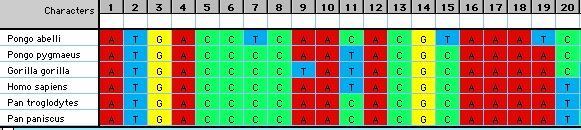
\includegraphics[width=\textwidth]{dna-ex}
}

\frame{
    \begin{tikzpicture}
        \node [rectangle,draw,align=left,x=0.4cm] (root) {
            \tl{py\alt<1>{\textcolor{tachameleon}}{}{vo}\alt<1>{}{\cur}}
            {\alt<1>{\textcolor{tachameleon}}{}vide\alt<1>{\textcolor{tachameleon}}{}o\alt<1>{}{\cur}}
        };

        \pause
        \pause

        \node [rectangle,draw,align=left,below=1 of root,scale=0.6] (b) { \tl{pyv\curc o}{vide\curc o} };

        \node [rectangle,draw,align=left,left=2.5 of b,scale=0.6] (a) { \tl{pyv\curc o}{video{\cur}} };

        \node [rectangle,draw,align=left,right=2.5 of b,scale=0.6] (c) { \tl{pyvo{\cur}}{vide\curc o} };

        \draw[->] (a) -- (root);
        \draw[->,thick] (b) -- (root);
        \draw[->] (c) -- (root);

        \pause

        \node [rectangle,draw,align=left,below=0.3 of a,scale=0.4] (ab) { \tl{py\curc vo}{video{\cur}} };
        \node [rectangle,draw,align=left,left=0.3 of ab,scale=0.4,fill=ta2aluminium] (aa) { \tl{py\curc vo}{vide\curc o} };
        \node [rectangle,draw,align=left,right=0.3 of ab,scale=0.4] (ac) { \tl{pyv{\cur}o}{vide\curc o} };
        \node [rectangle,draw,align=left,below=0.3 of b,scale=0.4] (bb) { \tl{py\curc vo}{vide{\cur}o} };
        \node [rectangle,draw,align=left,left=0.3 of bb,scale=0.4,fill=ta2aluminium] (ba) { \tl{py\curc vo}{vid\curc eo} };
        \node [rectangle,draw,align=left,right=0.3 of bb,scale=0.4] (bc) { \tl{pyv{\cur}o}{vid\curc eo} };
        \node [rectangle,draw,align=left,below=0.3 of c,scale=0.4] (cb) { \tl{pyv\curc o}{vid{\cur}eo} };
        \node [rectangle,draw,align=left,left=0.3 of cb,scale=0.4,fill=ta2aluminium] (ca) { \tl{py\curc vo}{vide\curc o} };
        \node [rectangle,draw,align=left,right=0.3 of cb,scale=0.4] (cc) { \tl{pyvo{\cur}}{vid\curc eo} };

        \foreach \r in {a,b,c} {
            \draw[->] (\r a) -- (\r);
            \draw[->] (\r b) -- (\r);
            \draw[->] (\r c) -- (\r);
        }

        \pause

        \foreach \r in {a,b,c} {
            \foreach \s in {a,b,c} {
                \node [rectangle,draw,align=left,below=0.3 of \r\s,scale=0.1] (\r\s b) { \tl{pyvo}{video} };
                \node [rectangle,draw,align=left,left=0.1 of \r\s b,scale=0.1] (\r\s a) { \tl{pyvo}{video} };
                \node [rectangle,draw,align=left,right=0.1 of \r\s b,scale=0.1] (\r\s c) { \tl{pyvo}{video} };

                \foreach \t in {a,b,c} {
                    \draw[->] (\r\s\t) -- (\r\s);

                    \node [align=left,below=0.1 of \r\s\t,scale=0.01] (\r\s\t b) { };
                    \node [align=left,left=0.1 of \r\s\t b,scale=0.01] (\r\s\t a) { };
                    \node [align=left,right=0.1 of \r\s\t b,scale=0.01] (\r\s\t c) { };

                    \foreach \u in {a,b,c} {
                        \draw (\r\s\t\u) -- (\r\s\t);
                    }
                }
            }
        }

    \end{tikzpicture}
}

\frame{
    \texttt{
    \begin{tikzpicture}
        %\renewcommand\pause{}
        \draw (0,0) grid (6,5);
        \node [below] at (1,0) {v\strut};
        \node [below] at (2,0) {i\strut};
        \node [below] at (3,0) {d\strut};
        \node [below] at (4,0) {e\strut};
        \node [below] at (5,0) {o\strut};
        %
        \node [left] at (0,1) {p\strut};
        \node [left] at (0,2) {y\strut};
        \node [left] at (0,3) {v\strut};
        \node [left] at (0,4) {o\strut};
        %
        \pause
        \node [rectangle,draw,align=left,scale=0.4] (n54) at (7,5) { \tl{pyvo{\cur}}{video{\cur}} };
        \draw[draw=ta3skyblue] (5.5,4.5) -- (n54);
        \pause
        \node [rectangle,draw,align=left,scale=0.4] (n53) at (7,4) { \tl{pyv{\cur}o}{video{\cur}} };
        \draw[draw=ta3skyblue] (5.5,3.5) -- (n53);
        \pause
        \node [rectangle,draw,align=left,scale=0.4] (n43) at (7,3) { \tl{pyv{\cur}o}{vide{\cur}o} };
        \draw[draw=ta3skyblue] (4.5,3.5) -- (n43);
        \pause
        \node [rectangle,draw,align=left,scale=0.4] (n44) at (4.5,6) { \tl{pyvo{\cur}}{vide{\cur}o} };
        \draw[draw=ta3skyblue] (4.5,4.5) -- (n44);
        \pause
        \node [rectangle,draw,align=left,scale=0.4] (n00) at (-1,-1) { \tl{{\cur}pyvo}{{\cur}video} };
        \draw[draw=ta3skyblue] (0.5,0.5) -- (n00);
        \pause
        \node [rectangle,draw,align=left,scale=0.4] (n10) at (1.5,-2) { \tl{{\cur}pyvo}{v{\cur}ideo} };
        \draw[draw=ta3skyblue] (1.5,0.5) -- (n10);
        %
        \pause
        \foreach \x in {1,...,5} {
            \foreach \y in {1,...,4} {
                \fill[draw=tascarletred] (\x,\y) +(-1pt,-1pt) -- +(+1pt,+1pt)
                                                 +(-1pt,+1pt) -- +(+1pt,-1pt);
            }
        }
        \fill[draw=ta3chameleon,fill=white] (1,3) circle [radius=2pt];
        \fill[draw=ta3chameleon,fill=white] (5,4) circle [radius=2pt];
        %
        \pause \node[xshift=0.5,yshift=0.5] at (0.5,0.5) { 0 };
        \pause \node[xshift=0.5,yshift=0.5] at (1.5,0.5) { 1 };
        \pause \node[xshift=0.5,yshift=0.5] at (2.5,0.5) { 2 };
        \pause \node[xshift=0.5,yshift=0.5] at (3.5,0.5) { 3 };
        \pause \node[xshift=0.5,yshift=0.5] at (4.5,0.5) { 4 };
        \pause \node[xshift=0.5,yshift=0.5] at (5.5,0.5) { 5 };
        %
        \pause
        \node [rectangle,draw,align=left,scale=0.4] (n01) at (-2,1.5) { \tl{p{\cur}yvo}{{\cur}video} };
        \draw[draw=ta3skyblue] (0.5,1.5) -- (n01);
        \pause
        \node [rectangle,draw,align=left,scale=0.4] (n02) at (-2,2.5) { \tl{py{\cur}vo}{{\cur}video} };
        \draw[draw=ta3skyblue] (0.5,2.5) -- (n02);
        %
        \pause \node[xshift=0.5,yshift=0.5] at (0.5,1.5) { 1 };
        \pause \node[xshift=0.5,yshift=0.5] at (0.5,2.5) { 2 };
        \pause \node[xshift=0.5,yshift=0.5] at (0.5,3.5) { 3 };
        \pause \node[xshift=0.5,yshift=0.5] at (0.5,4.5) { 4 };
        %
        \pause
        \node [rectangle,draw,align=left,scale=0.4] (n11) at (2.5,-1.5) { \tl{p{\cur}yvo}{v{\cur}ideo} };
        \draw[draw=ta3skyblue] (1.5,1.5) -- (n11);
        %
        \pause \node[xshift=0.5,yshift=0.5] at (1.5,1.5) { 2 };
        \pause \node[xshift=0.5,yshift=0.5] at (2.5,1.5) { 3 };
        \pause \node[xshift=0.5,yshift=0.5] at (3.5,1.5) { 4 };
        \pause \node[xshift=0.5,yshift=0.5] at (4.5,1.5) { 5 };
        \pause \node[xshift=0.5,yshift=0.5] at (5.5,1.5) { 6 };
        %
        \pause \node[xshift=0.5,yshift=0.5] at (1.5,2.5) { 3 };
        \pause \node[xshift=0.5,yshift=0.5] at (2.5,2.5) { 4 };
        \pause \node[xshift=0.5,yshift=0.5] at (3.5,2.5) { 5 };
        \pause \node[xshift=0.5,yshift=0.5] at (4.5,2.5) { 6 };
        \pause \node[xshift=0.5,yshift=0.5] at (5.5,2.5) { 7 };
        %
        \pause
        \node [rectangle,draw,align=left,scale=0.4] (n13) at (-2,3.5) { \tl{pyv{\cur}o}{v{\cur}ideo} };
        \draw[draw=ta3skyblue] (1.5,3.5) -- (n13);
        %
        \pause \node[xshift=0.5,yshift=0.5] at (1.5,3.5) { 2 };
        \pause \node[xshift=0.5,yshift=0.5] at (2.5,3.5) { 3 };
        \pause \node[xshift=0.5,yshift=0.5] at (3.5,3.5) { 4 };
        \pause \node[xshift=0.5,yshift=0.5] at (4.5,3.5) { 5 };
        \pause \node[xshift=0.5,yshift=0.5] at (5.5,3.5) { 6 };
        %
        \pause \node[xshift=0.5,yshift=0.5] at (1.5,4.5) { 3 };
        \pause \node[xshift=0.5,yshift=0.5] at (2.5,4.5) { 4 };
        \pause \node[xshift=0.5,yshift=0.5] at (3.5,4.5) { 5 };
        \pause \node[xshift=0.5,yshift=0.5] at (4.5,4.5) { 6 };
        \pause \node[xshift=0.5,yshift=0.5] at (5.5,4.5) { 5 };
        %
        \pause
        \begin{scope}[on background layer]%
            \alt<44->{ \fill[taaluminium,on background layer] (5,4) rectangle +(1,1); }{}%
            \alt<45->{ \fill[taaluminium,on background layer] (4,3) rectangle +(1,1); }{}%
            \alt<46->{ \fill[taaluminium,on background layer] (3,3) rectangle +(1,1); }{}%
            \alt<47->{ \fill[taaluminium,on background layer] (2,3) rectangle +(1,1); }{}%
            \alt<48->{ \fill[taaluminium,on background layer] (1,3) rectangle +(1,1); }{}%
            \alt<49->{ \fill[taaluminium,on background layer] (0,2) rectangle +(1,1); }{}%
            \alt<50->{ \fill[taaluminium,on background layer] (0,1) rectangle +(1,1); }{}%
            \alt<51->{ \fill[taaluminium,on background layer] (0,0) rectangle +(1,1); }{}%
        \end{scope}%
    \end{tikzpicture}
    }
}

\frame{
    \texttt{pyvo}

    \bigskip\bigskip\bigskip

    \texttt{vo}

    \bigskip\bigskip\bigskip

    \texttt{v\textcolor{tachameleon}{ide}o\textcolor{ta3aluminium}{!}}
}

\frame{}

\frame{
    \sk
    \textcolor{ta3gray}Dynamic {\textcolor{taskyblue}{Time Warping}\\
         \& Video Synchronization}
    \sk\sk
    \textcolor{ta2gray}{Petr Viktorin}\\[-0.25cm]
    \textcolor{ta2gray}{\tiny encukou@gmail.com}
    \sk
    \textcolor{ta2gray}{\tiny Brněnské PyVo, 2015-05-28}\\[-0.25cm]
}

\frame{
    Signal A:

    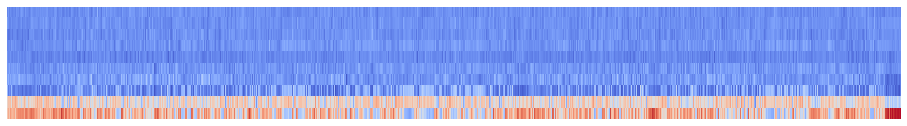
\includegraphics[width=\textwidth]{sig_a}

    Signal B:

    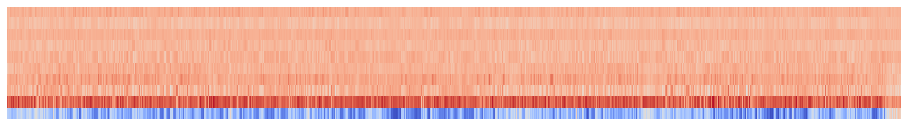
\includegraphics[width=\textwidth]{sig_b}
}

\frame{
    \begin{tikzpicture}[every node/.style={inner sep=0,outer sep=0}]
        \node[rotate=90,anchor=south west,scale=0.5] at (0,0)
            { 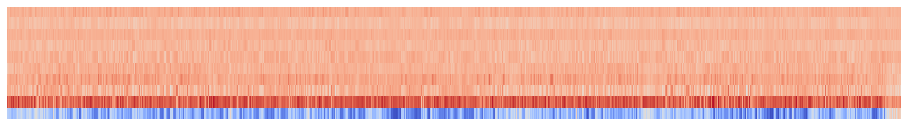
\includegraphics[width=\textwidth]{sig_b} };
        \node[anchor=south east,scale=0.5,rotate=180] at (0,0)
            { 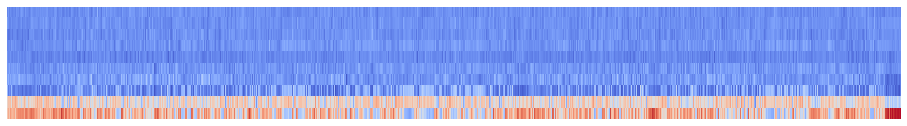
\includegraphics[width=\textwidth]{sig_a} };
        \pause
        \node[anchor=south west,scale=0.5] at (0,0)
            { 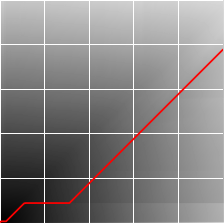
\includegraphics[width=0.7\textwidth]{result} };
        \pause
        \node[anchor=south west,scale=0.5] at (3,2.2)
            { 
\includegraphics[width=3cm]{nextwindow} };
        \pause
        \node[anchor=south west,scale=0.5] at (4,3.2)
            { 
\includegraphics[width=3cm]{nextwindow} };
    \end{tikzpicture}
}

\frame{
    \texttt{x - y}

    { 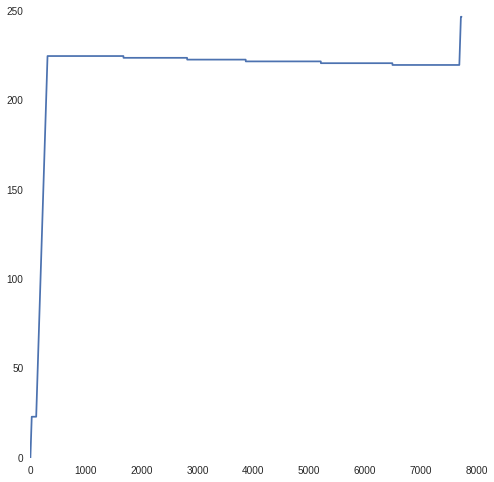
\includegraphics[width=8cm]{diff} }
}

\frame{
    \texttt{ffmpeg}
}

\frame{
    \begin{flushleft} 
    \setstretch{1}
    \fontsize{6pt}{7pt}\selectfont

    \texttt{
        \$ ffmpeg -filter\_complex [bd] anullsink  ; 
        color=color=00000000:duration=186.68:rate=50:size=1920x1081 [bb] ;
        movie=filename=in1.png:streams=dv [bc] ; 
        [bb][bc] overlay=repeatlast=1 [ay] ; [ay][az] overlay=repeatlast=0 [ax] ; [ax] setpts=expr=N/FRAME\_RATE/TB [out0] ;  
        color=color=00000000:duration=173.68:rate=50:size=1920x1080 [av] ;  
        movie=filename=in2.png:streams=dv [aw] ; 
        [av][aw] overlay=repeatlast=1 [au] ; [au] \alt<2->{\textcolor{ta2skyblue}}{}{fade=alpha=1}:color=00000000:duration=0.5:start\_time=173.18:type=out [ag] ; 
        movie=filename=in3.ogv:streams=dv+da [at][bd] ;
        [at] fps=fps=30 [as] ; [as] \alt<3->{\textcolor{ta2skyblue}}{}{format=pix\_fmts=rgba|yuva420p|yuva422p|yuva444p} [ar] ; [ar] setpts=expr=PTS-STARTPTS [aq] ;
        [aq] scale=h=1080:w=1440 [ap] ; [ap] setsar=sar=1 [ao] ; [ao] pad=color=00000000:h=1080:w=1920:x=0:y=0 [an] ; [an] fps=fps=25 [am] ;
        [am] fade=alpha=1:color=00000000:duration=0.5:start\_time=179.233333:type=out [al] ; [al] trim=start=5.24506890629 [ak] ;
        [ak] setpts=expr=PTS-STARTPTS [aj] ; [aj] trim=end=173.68 [ai] ; [ai] setpts=expr=PTS-STARTPTS [ah] ; [ag][ah] overlay=repeatlast=0 [w] ;
        [af] fps=fps=30 [ae] ; [ae] format=pix\_fmts=rgba|yuva420p|yuva422p|yuva444p [ad] ; [ad] setpts=expr=PTS-STARTPTS [ac] ;
        [ac] scale=h=271:w=481 [ab] ; [ab] setsar=sar=1 [aa] ; [aa] pad=color=00000000:h=1080:w=1920:x=1438:y=809 [z] ; [z] fps=fps=25 [y] ;
        [y] fade=alpha=1:color=00000000:duration=0.5:start\_time=173.18:type=out [x] ; [w][x] overlay=repeatlast=0 [b] ;
        movie=filename=in4.MTS:streams=dv+da [af][v] ;
        [v] asetpts=expr=PTS-STARTPTS [c] ;  color=color=00000000:duration=6:rate=50:size=1921x1081 [t] ;
        movie=filename=in5.png:streams=dv [u] ;
        [t][u] overlay=repeatlast=1 [s] ; [s] fade=alpha=1:color=00000000:duration=0.5:start\_time=0:type=in [r] ;
        [r] fade=alpha=1:color=00000000:duration=0.5:start\_time=5.5:type=out [d] ;  aevalsrc=duration=6:exprs=0 [e] ;
        color=color=00000000:duration=7:rate=50:size=1921x1081 [p] ;
        movie=filename=in6.png:streams=dv [q] ; 
        [p][q] overlay=repeatlast=1 [i] ;  color=color=00000000:duration=7:rate=50:size=528x528 [n] ;
        movie=filename=in7.png:streams=dv [o] ; 
        [n][o] overlay=repeatlast=1 [m] ; [m] scale=h=528:w=528 [l] ; [l] setsar=sar=1 [k] ; [k] pad=color=00000000:h=1080:w=1920:x=697:y=439 [j] ;
        [i][j] overlay=repeatlast=0 [h] ; [h] fade=alpha=1:color=00000000:duration=0.5:start\_time=0:type=in [f] ;  aevalsrc=duration=7:exprs=0 [g] ; 
        [b][c][d][e][f][g] concat=a=1:n=3:v=1 [az][a] ; [a] asetpts=expr=N/SR/TB [out1]
        -f mp4 -c:v libx264 -c:a aac -crf 30 -maxrate 5000k -strict -2 -map [out0] -map [out1]
        outfile.mp4
    }
    \end{flushleft} 
}

\end{center}
\end{document}

%% ffplay -f alsa -i hw:0
